\documentclass[conference]{IEEEtran}
\IEEEoverridecommandlockouts
% The preceding line is only needed to identify funding in the first footnote. If that is unneeded, please comment it out.
\usepackage{cite}
\usepackage{amsmath,amssymb,amsfonts}
\usepackage{algorithmic}
\usepackage{graphicx}
\usepackage{textcomp}
\usepackage{xcolor}
\def\BibTeX{{\rm B\kern-.05em{\sc i\kern-.025em b}\kern-.08em
    T\kern-.1667em\lower.7ex\hbox{E}\kern-.125emX}}
\begin{document}

\title{Emotion analysis in dataset}


\author{\IEEEauthorblockN{Meriem Aggoune}
\IEEEauthorblockA{\textit{dept. name of organization (of Aff.)} \\
\textit{name of organization (of Aff.)}\\
City, Country \\
email address or ORCID}
\and
\IEEEauthorblockN{ Lauri Heikka}
\IEEEauthorblockA{\textit{Faculty of Information Technology and Electrical Engineering} \\
\textit{Univ. of Oulu}\\
Oulu, Finland \\
lauri.heikka@student.oulu.fi}
\and
\IEEEauthorblockN{Anusha Ihalapathiranae}
\IEEEauthorblockA{\centerline{Faculty of Information Technology and Electrical Engineering} \\
\textit{Univ. of Oulu}\\
Oulu, Finland \\
anusha.ihalapathirana@student.oulu.fi}

}

\maketitle

\begin{abstract}
We document a series of experiments on using a variety of natural language processing methods to classify emotions conveyed by sentences. In particular, we compare word categorizations, semantic similarity approaches and machine learning approaches. The machine learning approaches consist of classification models based on bag-of-words representations and convolutional neural networks applied on word embeddings. Our results indicate that machine learning approaches outperform string matching and semantic similarity with a considerable margin. Within the machine learning approaches, convolutional neural networks with word embeddings provide an improvement in accuracy of around 3-5 percentage points over bag-of-words models. The best accuracy on a hold-out validation set, around 93\%, is achieved with a CNN approach using pre-trained word2vec embeddings. However, custom-trained word embeddings provide similar performance with less computational overhead.
\end{abstract}

\begin{IEEEkeywords}
natural language processing, text classification, sentiment analysis
\end{IEEEkeywords}

\section{Group info}
Group 10

Members: Meriem Aggoune, Lauri Heikka, Anusha Ihalapathiranae

Title: Emotion Analysis in Dataset

Github: https://github.com/MeriemLil/NLP\_Project

\section{Introduction}
Emotions are feelings that caused by a situation person interact with. It is also associate with person’s character, mood, personality and motivation. People express their feelings and emotions using verbally and non-verbally such as words, intonation of voice, facial expressions, gestures, and tears. Nowadays people tend to communicate their ideas, opinions, and feelings through social medias, Such as tweeter, facebook, instergram. People filled with lot emotions and they commonly use written text to express their emotions and feelings through social medias. Categorizing text into emotion types is known as emotion analysis. Sentiment analysis detect positive, negative, and neutral feelings from text and emotion analysis detect the types of feelings, emotion state, in the text \cite{emotiondetection}.

Emotion analysis takes major role in some applications which use emotion recognition, and it is a growing research area. There are supervised and unsupervised approaches can be found in this research area. A novel unsupervised context-based approach represents in \cite{unsupervisedemotiondetection} to detect emotions from text in sentence level. Their approached does not need any existing manually created lexicons and they used semantic relation between words and emotion type. They fine tune scores using syntactic dependencies within the sentence structure and proves this model provide more accurate results than other unsupervised approaches. Research carried out in \cite{jan2020emotion} paid their attention towards capturing semantic features in the text. Authors used distributional semantic model to calculate the semantic relatedness of the emotion in the text and they achieved accuracy of 71.79\% without training or annotation of data use.

A lot of research had been carried out on sentiment analysis and emotion analysis problem in many different languages. \cite{chaffaretal}  demonstrate their work on supervised machine learning approach to recognize the emotion types using emotion annotated dataset which combined news headlines, fairy tales and blogs. They use bag of words and N-grams and proved that support vector machines classifier shows better performance and generalization than the other classifiers they used. 

\cite{kim-2014-convolutional} introduce convolutional neural networkds for text categorization. Similar concepts are explored by e.g. \cite{johnsonetal} introduced a low complexity word level deep convolutional neural network for text categorization and \cite{dossantosetal} propose new convolutional neural network that exploits from character to sentence level information to perform sentiment analysis of short text such as tweeter messages. They found that combining small text with prior knowledge is effective.

Research in \cite{bert} introduced new language representation model, BERT, a pretrain deep bidirectional representations from unlabeled text. They used conditioning on both left and right context in all layers. BERT has achieved good results in many language understandings tasks. \cite{ bertclassification} used BERT on text classification and provide general solution for BERT fine tuning. Similarly, research on \cite{xu2020improving} improves the fine tuning of BERT using two effective mechanisms: self-ensemble and self-distillation.

In this research we are focusing on emotion analysis using word categorizations, semantic similarity approaches and machine learning approaches.
\section{Data and Methodologies}
\subsection{Datasets and sources}
Our main dataset of interest is a labeled dataset of 20 000 sentences with between 3 and 66 words. The dataset is provided by \cite{kaggledata}. The sentences are labeled to convey one of six different emotions: fear, anger, joy, love, surprise and sadness. The dataset is collected following the approach of \cite{saravia-etal-2018-carer}. The sentences are tweets, and the emotion labels are hashtags at the end of the tweet. The sentences are preprocessed in that they contain no punctuation or special characters and all words are lowercase.

The dataset has a predefined split into training, test and validation samples, with 16 000, 2 000 and 2 000, respectively. Because the semantic similarity and string matching approaches do not employ any predictive modeling, in these sections we use the all 20 000 sentences to measure prediction accuracy. For the machine learning approaches, we use the training set for model training, the test set for model selection and hyperparameter tuning, and reserve the validation dataset as a final benchmark, to ensure a fair comparison accross approaches.

In addition, we use pre-trained, 300-dimensional word2vec embeddings  from \cite{mikolov2013distributed} and pre-trained fastText embeddings from \cite{bojanowski2016enriching}. Both datasets consist of 300-dimensional word embeddings, with embeddings for 3 and 1 million english words, respectively. For the string matching, we use the Harvard General Inquirer dataset, which contains categorizations for around 11 000 english words.

\subsection{Harvard Inquirer and String Matching}
The first method we explore is to categorize each word in Harvard General Inquirer \cite{harvardgeneralinquirer} to each emotion type. We use a filtering technique to this categorization. To identify words related to love emotion, we include Harvard General Inquirer words with that are labeled Affil label and exclude words associated with Negative label. The categories used for all six labels is reported in Table~\ref{taba3}. We store this information into a database and then compute the occurrences of words associated with each label for each sentence and predict the label of a sentence to be the category with the highest number of words.

\subsection{Empath Client Categories}
The next method we explore is to use the Empath Client \cite{empathclient}, a text analyzing tool with pre-build category set, to compute empath category similarity by mapping labeled sentences in dataset and empath categories using the concept of common hypernymy. We also map using exact empath emotion category. However, considering the poor performance of these
\subsection{Semantic Similarity}
asd
\subsection{SentiStrength Sentiment Scores}
As part of the project specification, we also use the SentiStrength client \cite{sentistrength}, to compute sentiment scores. These can be potentially be used as an additional feature in any approach to distinguish between the negative and positive emotions. However, intuitively, the more difficult task is distinguishing between different positive emotions and between different negative emotions. For this purpose, the sentiment scores are unlikely to provide added benefit. Considering this, and the fact that the simple approaches perform quite poorly, we do not explore the effects of these sentiment scores onto the accuracy of different models. Sentiment scores are still delivered as part of the project database, as suggested in the project specification.

\section{Bag-of-Words Models}
asd
\subsection{Convolutional Neural Networks}

We replicate the convolutional neural network architecture used in \cite{kim-2014-convolutional}. The architecture is outlined in \ref{fig1}. Sentences are represented as $n\times k$ matrices of word vectors, where \emph{n} refers to the length of the sentences and $k$ to the dimension of the word vectors. All sentences are zero-padded to length $n$. Then a set of convolutions are applied on the sentences
\begin{equation}
c_i = f(w * x_{i:i+h-1} + b){eq1}
\end{equation}


A similar architecture is proposed in \cite{johnsonetal}, but one where sentences are not padded to a fixed length.  Note that, the application of max-pooling is likely to make the zero-padding inconsequential.

\begin{figure}[htbp]
\centerline{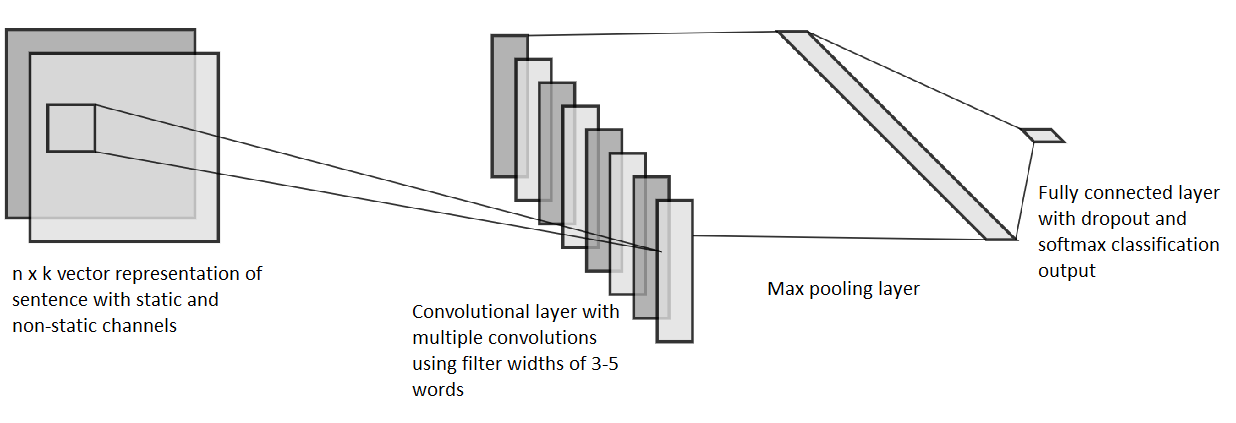
\includegraphics[width = 0.5 \textwidth]{fig1.png}}
\caption{Example of a figure caption.}
\label{fig1}
\end{figure}

In \cite{kim-2014-convolutional}, pre-trained Word2Vec embeddings from \cite{mikolov2013distributed} \cite{bojanowski2016enriching} are used. In addition to replicating this approach, we consider a few alternatives. First, we test pretrained fastText embeddings . Second, we explore explore training our own word2vec and fastText embeddings.
The word2vec model...
The fasttext model...
 For both models, we use a maximum distance between predicted words of five, and use early stopping on a word analogy evaluation task. 

We use sentence length $n = 70$ experiment with 50-, 100- and 300-dimensional word embeddings for the custom-trained word embeddings. With the pre-trained embeddings, we are restricted to the commonly available 300-dimensional word embeddings. In the convolution windo


\section{Results and Discussion}

\subsection{Word categorizations and semantic similarity}

\begin{table}[htbp]
\caption{Word categorizations and semantic similarity accuracies}
\begin{center}
\begin{tabular}{|c|c|}
\hline
\textbf{Classifier}&\multicolumn{1}{|c|}{\textbf{Accuracy}} \\ 

\hline
Harvard String Matching & 0.336 \\ 
\hline
Empath Client & 0.160 \\ 
\hline
Empath Client with exact categories & 0.183 \\ 
\hline
Semantic Similarity - One synset & 0.269 \\ 
\hline
Semantic Similarity - All synset & 0.240 \\ 
\hline
\end{tabular}
\label{tab1}
\end{center}
\end{table}

\subsection{Model selection for bag-of-words}
Table~\ref{tab5} reports the accuracies on the test dataset used for model selection.
\begin{table}[htbp]
\caption{Maximum accuracy on the test dataset across different bag-of-words setups}
\begin{center}
\begin{tabular}{|c|c|c|}
\hline
\textbf{}&\multicolumn{2}{|c|}{\textbf{}} \\ 
\cline{2-3}
\textbf{parameter} & \textbf{\textit{value}}& \textbf{\textit{score}} \\ 
\hline
vectorizer & CountVectorizer & 0.886 \\ 
\cline{2-3}
 & TfidfVectorizer & 0.888 \\ 
\hline
stopwords & nltk & 0.888 \\ 
\cline{2-3}
 & none & 0.878 \\ 
\cline{2-3}
 & sk & 0.884 \\ 
\hline
lemmatize & 0 & 0.888 \\ 
\cline{2-3}
 & 1 & 0.886 \\ 
\hline
max features  & 100 & 0.396 \\ 
\cline{2-3}
  & 500 & 0.728 \\ 
\cline{2-3}
 & 1000 & 0.865 \\ 
\cline{2-3}
  & 2000 & 0.880 \\ 
\cline{2-3}
  & 3000 & 0.886 \\ 
\hline
classifier & DecisionTreeClassifier & 0.866 \\ 
\cline{2-3}
 & GradientBoostingClassifier & 0.849 \\ 
\cline{2-3}
 & LogisticRegression & 0.878 \\ 
\cline{2-3}
 & MultinomialNB & 0.859 \\ 
\cline{2-3}
 & RandomForestClassifier & 0.888 \\ 
\cline{2-3}
 & SVC & 0.876 \\ 
\hline
\end{tabular}
\label{tab5}
\end{center}
\end{table}

\subsection{Validation set performance of best models}
Table~\ref{tab1} reports the accuracies on the test dataset used for model selection.

\begin{table}[htbp]
\caption{Validation and test set accuracies for best models}
\begin{center}
\begin{tabular}{|c|c|c|}
\hline
\textbf{}&\multicolumn{2}{|c|}{\textbf{Accuracy}} \\ 
\cline{2-3}
\textbf{Classifier} & \textbf{\textit{Validation}}& \textbf{\textit{Test}} \\ 
\hline
MultinomialNB & 0.681 & 0.694 \\ 
\hline
LogisticRegression & 0.872 & 0.864 \\ 
\hline
RandomForestClassifier & 0.899 & 0.89 \\ 
\hline
CNN fastText pretrained & 0.925 & 0.928 \\ 
\hline
CNN Word2Vec own & 0.928 & 0.929 \\ 
\hline
CNN fastText own & 0.928 & 0.931 \\ 
\hline
CNN Word2Vec pretrained & 0.930 & 0.928 \\ 
\hline
\end{tabular}
\label{tab1}
\end{center}
\end{table}

\begin{table}[htbp]
\caption{Validation precision and recall for best models}
\begin{center}
\begin{tabular}{|c|c|c|}
\hline
\textbf{}&\multicolumn{2}{|c|}{\textbf{Metric}} \\ 
\cline{2-3}
\textbf{Classifier} & \textbf{\textit{Precision}}& \textbf{\textit{Recall}} \\ 
\hline
MultinomialNB & 0.734 & 0.681 \\ 
\hline
LogisticRegression & 0.875 & 0.872 \\ 
\hline
RandomForestClassifier & 0.898 & 0.899 \\ 
\hline
CNN fastText pretrained & 0.926 & 0.925 \\ 
\hline
CNN Word2Vec own & 0.93 & 0.928 \\ 
\hline
CNN fastText own & 0.928 & 0.928 \\ 
\hline
CNN word2vec pretrained & 0.930 & 0.930 \\ 
\hline
\end{tabular}
\label{tab2}
\end{center}
\end{table}



\section{Overall discussion and related literature}
...

As mentioned in the introduction, the state of the art for text classification tasks has moved beyond word level embedding representations considered here. For example, \cite{bert}, \cite{xlnet} and \cite{bertclassification} employ pre-trained bidirectional encoder representations to achieve state-of-the-art results in sentence classification. However, constructing a replication and a fair comparison of these models is beyond the scope of this study.
\footnote{There is a minimal, unofficial implementation of BERT\cite{bert} embeddings on the dataset we study\cite{kaggledata} available at Kaggle by the dataset author. This implementation appears to exceed the accuracy of the best studied CNN model by around 0.3 percentage units.}
Exploring alternative setups for training the word vectors is likewise beyond the scope of this paper.

The pretrained embeddings are quite large in size, while custom embeddings trained on the emotions dataset are much smaller. Furthermore, because model performance with embeddings trained on the emotions dataset is very close in performance to the pretrained embeddings, the custom models provide a lightweight alternative for model serving. It is important to note, however, that the emotions dataset contains very homogenous sentences across the training, test and validation datasets. This causes the vocabulary of the custom word embeddings to be much smaller than the pretrained word embeddings. Therefore the model is more likely to suffer in performance on out-of-distribution sentences.

...
\section{Conclusion}
conclude.

\section{Latex examples}

To be removed.

\subsection{Equations example}
\begin{equation}
a+b=\gamma\label{eq}
\end{equation}

Use ``\eqref{eq}'', not ``Eq.~\eqref{eq}'' or ``equation \eqref{eq}'', except at 
the beginning of a sentence: ``Equation \eqref{eq} is . . .''

\subsection{Some Common Mistakes}\label{SCM}
\begin{itemize}
\item The word ``data'' is plural, not singular.
\item In your paper title, if the words ``that uses'' can accurately replace the word ``using'', capitalize the ``u''; if not, keep using lower-cased.
\item Be aware of the different meanings of the homophones ``affect'' and ``effect'', ``complement'' and ``compliment'', ``discreet'' and ``discrete'', ``principal'' and ``principle''.
\item Do not confuse ``imply'' and ``infer''.
\item The prefix ``non'' is not a word; it should be joined to the word it modifies, usually without a hyphen.
\item There is no period after the ``et'' in the Latin abbreviation ``et al.''.
\item The abbreviation ``i.e.'' means ``that is'', and the abbreviation ``e.g.'' means ``for example''.
\end{itemize}




\section*{Acknowledgment}

We thank Mourad Oussalah and other seminar participants for their helpful comments during
 the Natural Language Processing and Text Mining course project seminar.

\bibliographystyle{./IEEEtran}
\bibliography{./paper}

\appendices
\section{Additional Tables}
\label{FirstAppendix}

\begin{table}[htbp]
\caption{Average accuracy across different bag-of-words setups}
\begin{center}
\begin{tabular}{|c|c|c|}
\hline
\textbf{}&\multicolumn{2}{|c|}{\textbf{}} \\ 
\cline{2-3}
\textbf{parameter} & \textbf{\textit{value}}& \textbf{\textit{score}} \\ 
\hline
vectorizer & CountVectorizer & 0.719 \\ 
\cline{2-3}
 & TfidfVectorizer & 0.727 \\ 
\hline
stopwords & nltk & 0.725 \\ 
\cline{2-3}
 & none & 0.703 \\ 
\cline{2-3}
 & sk & 0.74 \\ 
\hline
lemmatize & 0 & 0.723 \\ 
\cline{2-3}
 & 1 & 0.723 \\ 
\hline
max features & 100.0 & 0.361 \\ 
\cline{2-3}
 & 500.0 & 0.631 \\ 
\cline{2-3}
 & 1000.0 & 0.830 \\ 
\cline{2-3}
 & 2000.0 & 0.844 \\ 
\cline{2-3}
 & 3000.0 & 0.845 \\ 
\hline
classifier & DecisionTreeClassifier & 0.702 \\ 
\cline{2-3}
 & GradientBoostingClassifier & 0.729 \\ 
\cline{2-3}
 & LogisticRegression & 0.733 \\ 
\cline{2-3}
 & MultinomialNB & 0.704 \\ 
\cline{2-3}
 & RandomForestClassifier & 0.744 \\ 
\cline{2-3}
 & SVC & 0.723 \\ 
\hline
\end{tabular}
\label{taba5}
\end{center}
\end{table}



\begin{table}[htbp]
\caption{Best CNN Model by Mode}
\begin{center}
\begin{tabular}{|c|c|c|c|}
\hline
\textbf{}&\multicolumn{3}{|c|}{\textbf{Metric}} \\ 
\cline{2-4}
\textbf{name} & \textbf{\textit{mode}}& \textbf{\textit{Accuracy}}& \textbf{\textit{Loss}} \\ 
\hline
CNN Word2Vec own & multichannel & 0.927 & 6.404 \\ 
\cline{2-4}
 & non-static & 0.929 & 6.44 \\ 
\cline{2-4}
 & static & 0.900 & 10.404 \\ 
\hline
CNN fastText own & multichannel & 0.921 & 9.463 \\ 
\cline{2-4}
 & non-static & 0.931 & 6.599 \\ 
\cline{2-4}
& static & 0.770 & 25.254 \\ 
\hline
CNN fastText pretrained & multichannel & 0.928 & 6.326 \\ 
\cline{2-4}
 & non-static & 0.928 & 6.133 \\ 
\cline{2-4}
 & static & 0.908 & 8.786 \\ 
\hline
CNN word2vec pretrained & multichannel & 0.928 & 6.583 \\ 
\cline{2-4}
& non-static & 0.927 & 6.668 \\ 
\cline{2-4}
& static & 0.906 & 9.025 \\ 
\hline
\end{tabular}
\label{taba1}
\end{center}
\end{table}

\begin{table}[htbp]
\caption{Hyperparameters for the best CNN Models}
\begin{center}
\begin{tabular}{|c|c|c|c|c|}
\hline
\textbf{}&\multicolumn{4}{|c|}{\textbf{Metric}} \\ 
\cline{2-5}
\textbf{Hyperparameter} & \textbf{\textit{CNN fastText pretrained}}& \textbf{\textit{CNN Word2Vec own}}& \textbf{\textit{CNN fastText own}}& \textbf{\textit{CNN word2vec pretrained}} \\ 
\hline
dev acc & 0.928 & 0.929 & 0.931 & 0.928 \\ 
\hline
dropout & 0.5 & 0.75 & 0.75 & 0.7 \\ 
\hline
num feature maps & 100.0 & 150.0 & 100.0 & 100.0 \\ 
\hline
regularization & 0.0 & 0.001 & 0.001 & 0.0 \\ 
\hline
word dim & 300.0 & 50.0 & 50.0 & 300.0 \\ 
\hline
\end{tabular}
\label{taba4}
\end{center}
\end{table}

\begin{table}[htbp]
\caption{Confusion matrices}
\begin{center}
\begin{tabular}{|c|c|c|c|c|c|c|}
\hline
\textbf{}&\multicolumn{6}{|c|}{\textbf{Label}} \\ 
\cline{2-7}
\textbf{Classifier} & \textbf{\textit{joy}}& \textbf{\textit{sadness}}& \textbf{\textit{anger}}& \textbf{\textit{fear}}& \textbf{\textit{love}}& \textbf{\textit{surprise}} \\ 
\hline
CNN Word2Vec & 664    32 & 525    26 & 254    16 & 196    34 & 158    30 & 60    5 \\ 

own & 40    1264 & 25    1424 & 21    1709 & 16    1754 & 20    1792 & 21    1914 \\ 
\hline
CNN fastText & 674    38 & 531    32 & 258    25 & 171    12 & 155    22 & 67    15 \\ 

own & 30    1258 & 19    1418 & 17    1700 & 41    1776 & 23    1800 & 14    1904 \\ 
\hline
CNN fastText & 664    36 & 520    17 & 259    24 & 195    35 & 148    27 & 64    11 \\ 

pretrained & 40    1260 & 30    1433 & 16    1701 & 17    1753 & 30    1795 & 17    1908 \\ 
\hline
CNN word2vec & 673    36 & 524    29 & 255    15 & 189    27 & 156    23 & 64    9 \\ 

pretrained & 31    1260 & 26    1421 & 20    1710 & 23    1761 & 22    1799 & 17    1910 \\ 
\hline
LogisticRegression & 672    119 & 516    73 & 229    23 & 155    23 & 122    10 & 51    7 \\ 

 & 32    1177 & 34    1377 & 46    1702 & 57    1765 & 56    1812 & 30    1912 \\ 
\hline
MultinomialNB & 683    364 & 514    268 & 93    3 & 60    3 & 12    0 & 0    0 \\ 

 & 21    932 & 36    1182 & 182    1722 & 152    1785 & 166    1822 & 81    1919 \\ 
\hline
RandomForestClassifier & 659    72 & 508    43 & 241    21 & 185    36 & 142    21 & 62    10 \\ 

 & 45    1224 & 42    1407 & 34    1704 & 27    1752 & 36    1801 & 19    1909 \\ 
\hline
\end{tabular}
\label{taba2}
\end{center}
\end{table}

\begin{table}[htbp]
\caption{Harvard General Inquirer Category Selection}
\begin{center}
\begin{tabular}{|c|c|c|}
\hline
\textbf{}&\multicolumn{2}{|c|}{\textbf{Inclusion}} \\ 
\cline{2-3}
\textbf{Label} & \textbf{\textit{Included}}& \textbf{\textit{Excluded}} \\
\hline
surprise & Arousal & \\
\hline
joy & Positiv & Affil \\
\hline
love & Affil & Negativ\\
\hline
anger & Hostile & \\
\hline
sadness & Negativ & Hostile\\
\hline
fear & Weak & \\
\hline
\end{tabular}
\label{taba3}
\end{center}
\end{table}

\label{FirstAppendix}

\end{document}
